% !TEX encoding = UTF-8 Unicode
%\documentclass[a4paper,11pt,spanish, twoside, openany]{tfg-uam-matematicas_25-26} 
\documentclass[a4paper,11pt,spanish, twoside]{tfg-uam-matematicas_25-26} 

\usepackage{customstyle}
\usepackage[utf8]{inputenc}
\usepackage{amsfonts, amssymb, amsmath, amsthm}
\usepackage{graphicx}
\usepackage{color}

% \newtheorem{teo}{Teorema}[chapter]
% \newtheorem{lema}[teo]{Lema}
% \newtheorem*{teo}{Teorema}


% \theoremstyle{definition}
% \newtheorem{defin}[teo]{Definición}

\title{Título del trabajo va aquí}
\author{Nombre y Apellidos del autor/a}
\curso{2025-2026}


%%%%%METADATOS: rellenar la info solicitada entre llaves
\usepackage{hyperref}
\hypersetup{
	pdfinfo={
            Title={ }, %Titulo del trabajo; ejemplo: Matematicas y desarrollo
            Author={ }, %Autor del trabajo. 
            Director1={ }, %Tutor1: en formato nombre.apellido, tal como aparece en la primera parte, antes de la arroba,  de su dirección de correo electrónico de la UAM; ejemplo: fernando.soria
            Director2={ }, %Tutor2: en formato nombre.apellido, tal como aparece en la primera parte, antes de la arroba,  de su dirección de correo electrónico de la UAM
            Ndirectores={ }, %Numero total de directores: 1 ó 2
            Tipo={TFG}, %no tocar
            Curso={2025-26}, %no tocar
            Palabrasclave={ },% Palabras clave del trabajo, separadas por comas y sin acentos ni espacios; ejemplo: morfismos, formas modulares, ecuaciones elipticas
				}
}
%%%%%%%%%%%%%%%%%%%%%%%%%%%%%%%

\begin{document}
    \frontmatter
    % Agradecimientos (Opcional)
    \cleardoublepage
    \null
    \vfill
    \begin{flushright}
        \textit{A todos los que me quieren.}
    \end{flushright}
    \vfill
    \cleardoublepage
    %%Fin de agradecimientos

    %%Resumen, en español y en inglés (Obligatorios ambos)
    % ------------------------------------------------------------------------------
% Esquema breve del abstract
% - Tema y contexto (productos finitos de Blaschke y disco unidad).
% - Objetivos y resultados principales (geometria hiperbolica, caracterizaciones,
%   valencia, aproximacion).
% - Enfoque/metodos (Schwarz--Pick, transformaciones de Möbius, argumentos de borde).
% ------------------------------------------------------------------------------
\begin{abstract}[spanish]
Este trabajo estudia los productos finitos de Blaschke como objetos centrales en la teoría de funciones holomorfas en el disco unidad. Se describe la geometría hiperbólica asociada a las métricas pseudohiperbólica y de Poincaré, con especial atención a sus isometrías y geodésicas, y se analizan consecuencias del lema de Schwarz--Pick para la clase de Schur y los automorfismos del disco. Se obtienen caracterizaciones de los productos finitos de Blaschke mediante condiciones de borde y representaciones racionales, junto con resultados de unicidad y valencia. Finalmente, se presentan teoremas de aproximación en la clase de Schur y en el álgebra del disco, así como versiones de Rouché y criterios recíprocos ligados a la distribución de ceros. La exposición combina técnicas de transformaciones de Möbius, principios de máximo y argumentos geométricos.
\end{abstract}


% ------------------------------------------------------------------------------
% Abstract outline (English)
% - Topic and context (finite Blaschke products on the unit disk).
% - Main goals/results (hyperbolic geometry, characterizations, valency, approximation).
% - Methods (Schwarz--Pick, Möbius maps, boundary arguments).
% ------------------------------------------------------------------------------
\begin{abstract}[english]
This work studies finite Blaschke products as fundamental objects in the theory of holomorphic functions on the unit disk. We develop the hyperbolic geometry associated with the pseudohyperbolic and Poincaré metrics, emphasize their isometries and geodesics, and analyze consequences of the Schwarz--Pick lemma for the Schur class and disk automorphisms. We obtain characterizations of finite Blaschke products via boundary conditions and rational representations, together with results on uniqueness and valency. Finally, we present approximation theorems in the Schur class and in the disk algebra, along with Rouché-type results and converse criteria related to the distribution of zeros. The exposition combines Möbius transformations, maximum principles, and geometric arguments.
\end{abstract}
    \cleardoublepage

    % Lista de símbolos (Opcional)
    % Título con mismo estilo que \chapter
    \begin{flushright}
        \Huge\bf Lista de símbolos\\*[-.5\baselineskip]
        \hrulefill
    \end{flushright}

    \begin{tabular}{ll}
        $\in$ & Pertenece a \\
        $\notin$ & No pertenece a \\
        $\subseteq$ & Subconjunto de \\
        $\subset$ & Subconjunto propio de \\
        $\cup$ & Unión de conjuntos \\
        $\cap$ & Intersección de conjuntos \\
        $\emptyset$ & Conjunto vacío \\
        $\mathbb{N}$ & Conjunto de números naturales \\
        $\mathbb{Z}$ & Conjunto de números enteros \\
        $\mathbb{Q}$ & Conjunto de números racionales \\
        $\mathbb{R}$ & Conjunto de números reales \\
        $\mathbb{C}$ & Conjunto de números complejos \\
        $f: A \to B$ & Función de $A$ en $B$ \\
        $\mathrm{Id}$ & Identidad \\
        $\ker(f)$ & Núcleo de una aplicación \\
        $\mathrm{Im}(f)$ & Imagen de una aplicación \\
        $\|x\|$ & Norma de un vector \\
        $\langle x,y \rangle$ & Producto interno \\
        $|A|$ & Cardinal de $A$ \\
        $\forall$ & Para todo \\
        $\exists$ & Existe \\
        $\Rightarrow$ & Implica \\
        $\Leftrightarrow$ & Equivalencia (si y sólo si) \\
        $\sum_{i=1}^n a_i$ & Suma finita \\
        $\prod_{i=1}^n a_i$ & Producto finito \\
        $\lim_{x \to a} f(x)$ & Límite de $f$ en $a$ \\
        $f'(x)$ & Derivada de $f$ \\
        $\int_a^b f(x)\,dx$ & Integral definida \\
        $O(g(n))$ & Cota asintótica superior \\
        $\cong$ & Isomorfismo \\
        $\simeq$ & Equivalencia \\
        $\approx$ & Aproximadamente igual \\
        $\triangleq$ & Definido como \\
        $\mathbb{P}(A)$ & Probabilidad del suceso $A$ \\
        $\mathbb{E}[X]$ & Esperanza de $X$ \\
        $\mathrm{Var}(X)$ & Varianza de $X$ \\
    \end{tabular}
    \cleardoublepage

    %%%%%%%%%%%%%%%%%%%%%%%%%%%%%%%%%%%%%%%%%%%%%%%%%%
    %%%%%%%%%%%%%%%%%%%%%%%%%%%%%%%%%%%%%%%%%%%%%%%%%%
    \mainmatter

    %%%A partir de aquí el cuerpo del trabajo  %%%%%%%
    \chapter*{Introducción}  % Capítulo sin numeración
\addcontentsline{toc}{chapter}{Introducción}  % Agrega la introducción al índice

%COMPLETAR mencionar que a veces para ahorrar espacio se omiten demostraciones o se dejan como ejercicios

    \chapter{El primer capítulo}\label{chap1}

% \clearpage


    \chapter{Geometría hiperbólica}\label{chap2}

\begin{defn}[Invariancia conforme]\label{defn:fn-invariante-conforme}
    Sea $F \colon \mathbb{D}^n \to \R$ una aplicación, diremos que $F$ es \emph{invariante conforme} si satisface que $\forall f \in \mathrm{Aut}(\mathbb{D}) : \forall z_1, \ldots, z_n \in \mathbb{D} : F(f(z_1), \ldots, f(z_n)) = F(z_1, \ldots, z_n)$.
\end{defn}

\section{Métrica pseudohiperbólica}

La métrica euclídea en el disco unidad no es completa (basta con tomar la sucesión de Cauchy dada por $z_n = 1 - \frac{1}{n}$ que no converge en $\mathbb{D}$) y no es invariante conforme. %REVISAR: comprobar esto con un ejemplo

Esto sugiere la necesidad de definir una métrica alternativa que sí satisfaga estas propiedades. El \exhyperref[teo:schwarz-pick]{teo-schwarz-pick}{teorema de Schwarz-Pick} proporciona un punto de partida, ya que asegura que para $f \in \mathrm{Aut}(\mathbb{D})$, $\forall z, w \in \mathbb{D} : \abs{\tau_{f(w)}(f(z))} = \abs{\tau_w(z)}$, es decir, la aplicación $\varrho \colon \mathbb{D} \times \mathbb{D} \to \R$ dada por $\varrho(z, w) \defeq \abs{\tau_w(z)}$ es invariante conforme. El objetivo de esta sección es demostrar que $\varrho$ es además una métrica completa en $\mathbb{D}$, que llamaremos \emph{métrica pseudohiperbólica}. Para ello, es conveniente entender mejor su geometría.

Denotaremos por $B_{\varrho}(z, r)$ a la bola abierta centrada en $z$ y de radio $r$ respecto a la métrica pseudohiperbólica. Es decir, $\forall z \in \mathbb{D}, r > 0 : B_{\varrho}(z, r) \defeq \left\{w \in \mathbb{D} : \varrho(z, w) < r\right\}$.

%Mantener
\begin{prop}[Bolas pseudohiperbólicas]\label{prop:bola-pseudohiperbolica-bola-euclidea}
    Sea $z \in \mathbb{D}$ y $r > 0$, entonces
    \[
    B_{\varrho}(z, r) = D\left(\frac{1 - r^2}{1 - r^2\abs{z}^2}\, z,\, \frac{1 - \abs{z}^2}{1 - r^2\abs{z}^2} \, r\right) \subset \mathbb{D}.
    \]
\end{prop}
\begin{dem}
    Por definición, $B_{\varrho}(z, r) = \exhyperref[defn:involucion-disco-unidad]{involucion-disco-unidad}{\tau_z}^{-1}(D(0, r)) = \tau_z(D(0, r))$ (\excref[lem:involucion-disco-unidad]{lem-involucion-disco-unidad}). Como $\tau_z$ es una \exhyperref[defn:transformacion-mobius]{transformacion-mobius}{transformación de Möbius}, por el \excref[teo:transformacion-mobius-circunferencias-generalizadas]{transformacion-mobius-circunferencias-generalizadas}, $B_{\varrho}(z, r)$ es un disco euclídeo. Es decir, $\exists w \in \mathbb{D}, s > 0 : B_{\varrho}(z, r) = \tau_{z}(D(0, r)) = D(w, s)$.

    Como el diámetro del disco unidad $\gamma \defeq \left\{t \, z/\abs{z} : t  \in (-1,1)\right\} \subset \mathbb{D}$ se mantiene invariante por $\tau_z$ %ORDENAR: referenciar
    y es una recta perpendicular a $\partial D(0, r)$, $\tau_z(\gamma) = \gamma$ es también perpendicular a $\tau_z(\partial D(0, r)) = \partial D(w, s)$ (ya que $\tau_z$ es conforme). Por tanto, $w \in \gamma$ estará en el punto medio entre $w_m = \tau_z\left(r \, z/\abs{z}\right)$ y $w_M = \tau_z\left(-r \, z/\abs{z}\right)$, es decir, $w = \frac{1}{2}(w_m + w_M)$. Operando, obtenemos que
    \[
    w_m = \tau_z\left(r \, \frac{z}{\abs{z}}\right) = \frac{z - r \, \frac{z}{\abs{z}}}{1 - \bar{z} r \, \frac{z}{\abs{z}}} = \frac{z (1 - r/\abs{z})}{1 - r \abs{z}} \cdot \frac{\abs{z}}{\abs{z}} = \frac{\abs{z} - r}{1 - r \abs{z}} \cdot \frac{z}{\abs{z}} = \tau_{\abs{z}}\left(r\right) \cdot \frac{z}{\abs{z}}. 
    \]
    y, de forma análoga, $w_M = \frac{\abs{z} + r}{1 + r \abs{z}} \cdot \frac{z}{\abs{z}} = \tau_{\abs{z}}(-r) \cdot \frac{z}{\abs{z}}$. Por tanto,
    \[
    w = \frac{w_m + w_M}{2} = \frac{1}{2} \left(\tau_{\abs{z}}(r) + \tau_{\abs{z}}(-r)\right) \cdot \frac{z}{\abs{z}} = \frac{1 - r^2}{1 - r^2 \abs{z}^2} \, z.
    \]

    Finalmente, $s$ viene dado por $\ds s = \abs{w - w_m} = \frac{1-\abs{z}^2}{1 - r^2 \abs{z}^2} \, r$.%REVISAR a lo mejor escribir las cuentas más detalladamente
    \hfill\qedsymbol
\end{dem}

%Quiza incluir en la presentación y citar el libro
\begin{figure}[ht]
    \centering
    \begin{subfigure}[b]{0.45\textwidth}
        \centering
        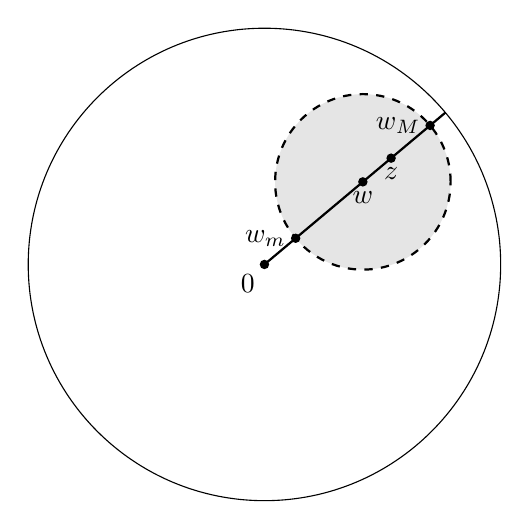
\begin{tikzpicture}[scale=3]
            % Parámetros ajustables: |z|, r y dirección (ángulo en grados)
            \def\absz{0.7}   % |z| \in (0,1)
            \def\r{0.6}      % r \in (0,1)
            \def\theta{40}   % dirección de z/|z|

            % Cálculos auxiliares
            \pgfmathsetmacro{\wm}{(\absz - \r)/(1 - \r*\absz)}
            \pgfmathsetmacro{\wM}{(\absz + \r)/(1 + \r*\absz)}
            \pgfmathsetmacro{\w}{\absz*(1 - \r*\r)/(1 - \r*\r*\absz*\absz)}
            \pgfmathsetmacro{\s}{((1 - \absz*\absz)/(1 - \r*\r*\absz*\absz))*\r}

            % Borde del disco unidad
            \draw (0,0) circle [radius=1];

            % Disco imagen por tau_z: centro w y radio s (relleno gris claro primero para no tapar puntos)
            \fill[gray!20] ({\w*cos(\theta)},{\w*sin(\theta)}) circle [radius=\s];

            % Segmento radial { t z/|z| : 0 < t < 1 }
            \draw[thick] (0,0) -- ({cos(\theta)},{sin(\theta)});

            % Origen
            \fill (0,0) circle (0.02) node[below left] {$0$};

            % Punto z (variable: |z|=\absz y dirección \theta)
            \fill ({\absz*cos(\theta)},{\absz*sin(\theta)}) circle (0.02) node[below] {$z$};

            % Puntos w_m, w, w_M sobre la dirección z/|z|
            \fill ({\wm*cos(\theta)},{\wm*sin(\theta)}) circle (0.02) node[left] {$w_m$};
            \fill ({\w*cos(\theta)},{\w*sin(\theta)})   circle (0.02) node[below] {$w$};
            \fill ({\wM*cos(\theta)},{\wM*sin(\theta)}) circle (0.02) node[left] {$w_M$};

            % Borde dashed del disco imagen
            \draw[dashed, thick] ({\w*cos(\theta)},{\w*sin(\theta)}) circle [radius=\s];
        \end{tikzpicture}
        \caption{Caso 1: $r \leq |z|$}
        \label{fig:caso1}
    \end{subfigure}
    \hfill
    \begin{subfigure}[b]{0.45\textwidth}
        \centering
        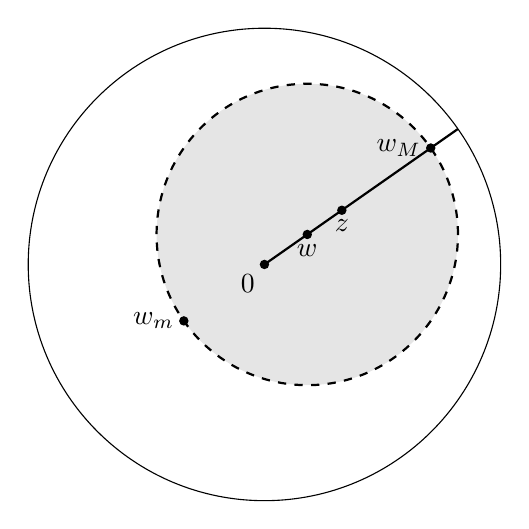
\begin{tikzpicture}[scale=3]
            % Parámetros ajustables: |z|, r y dirección (ángulo en grados)
            \def\absz{0.4}   % |z| \in (0,1)
            \def\r{0.7}      % r \in (0,1)
            \def\theta{35}   % dirección de z/|z|

            % Cálculos auxiliares
            \pgfmathsetmacro{\wm}{(\absz - \r)/(1 - \r*\absz)}
            \pgfmathsetmacro{\wM}{(\absz + \r)/(1 + \r*\absz)}
            \pgfmathsetmacro{\w}{\absz*(1 - \r*\r)/(1 - \r*\r*\absz*\absz)}
            \pgfmathsetmacro{\s}{((1 - \absz*\absz)/(1 - \r*\r*\absz*\absz))*\r}

            % Borde del disco unidad
            \draw (0,0) circle [radius=1];

            % Disco imagen por tau_z: centro w y radio s (relleno gris claro primero para no tapar puntos)
            \fill[gray!20] ({\w*cos(\theta)},{\w*sin(\theta)}) circle [radius=\s];

            % Segmento radial { t z/|z| : 0 < t < 1 }
            \draw[thick] (0,0) -- ({cos(\theta)},{sin(\theta)});

            % Origen
            \fill (0,0) circle (0.02) node[below left] {$0$};

            % Punto z (variable: |z|=\absz y dirección \theta)
            \fill ({\absz*cos(\theta)},{\absz*sin(\theta)}) circle (0.02) node[below] {$z$};

            % Puntos w_m, w, w_M sobre la dirección z/|z|
            \fill ({\wm*cos(\theta)},{\wm*sin(\theta)}) circle (0.02) node[left] {$w_m$};
            \fill ({\w*cos(\theta)},{\w*sin(\theta)})   circle (0.02) node[below] {$w$};
            \fill ({\wM*cos(\theta)},{\wM*sin(\theta)}) circle (0.02) node[left] {$w_M$};

            % Borde dashed del disco imagen
            \draw[dashed, thick] ({\w*cos(\theta)},{\w*sin(\theta)}) circle [radius=\s];
        \end{tikzpicture}
        \caption{Caso 2: $r > |z|$}
        \label{fig:caso2}
    \end{subfigure}
    \caption{Borde de $\mathbb{D}$, segmento radial en dirección $z/\lvert z\rvert$, y $B_{\varrho}(z,r)=\tau_z(D(0,r))$ con centro $w$ y radio $s$; se señalan $w_m$ y $w_M$.}
    \label{fig:bolas-pseudohiperbolicas}
\end{figure}

\subsection{Desigualdad triangular generalizada}

\begin{lem}%[]\label{lem:}
    Sea $z \in \mathbb{D}$ y $r \in (0,1)$, entonces
    \[
    \forall w \in \bar{B_{\varrho}(z, r)} : \frac{\abs{z}-r}{1 - r \abs{z}} \leq \abs{w} \leq \frac{\abs{z} + r}{1 + r \abs{z}}.
    \]
\end{lem}
\begin{dem}
    Por la \excref[prop:bola-pseudohiperbolica-bola-euclidea]{prop-bola-pseudohiperbolica-bola-euclidea}, $w_m = \frac{\abs{z} - r}{1 - r \abs{z}} \cdot \frac{z}{\abs{z}}$ y $w_M = \frac{\abs{z} + r}{1 + r \abs{z}} \cdot \frac{z}{\abs{z}}$ son los puntos de $\bar{B_{\varrho}(z, r)}$ más cercanos y más alejados del origen respectivamente (ver la \autoref{fig:bolas-pseudohiperbolicas}), luego el resultado se sigue de la desigualdad triangular de $\abs{\cdot}$.\hfill\qedsymbol
\end{dem}

\begin{cor}%[]\label{cor:}
    Sean $z_1, z_2 \in \mathbb{D}$, entonces
    \begin{enu}[2][label=\textnormal{(\arabic*)}]
        \item $\ds \frac{z_1 - z_2}{1 - \overline{z_1} z_2}  \in \partial B_{\exhyperref[defn:metrica-pseudohiperbolica-disco-unidad]{metrica-pseudohiperbolica-disco-unidad}{\varrho}}\left(z_1, \abs{z_2}\right)$
        \item $\ds \frac{\abs{z_1} - \abs{z_2}}{1 - \abs{z_1 \, z_2}} \leq \abs{\frac{z_1 - z_2}{1 - \overline{z_1} z_2}} \leq \frac{\abs{z_1} + \abs{z_2}}{1 + \abs{z_1\, z_2}}$.
    \end{enu}
\end{cor}
\begin{dem}
    \begin{enumerate}[label=\textnormal{(\arabic*)}]
        \item Basta ver que $\varrho \left(\exhyperref[lem:involucion-disco-unidad]{lem-involucion-disco-unidad}{\tau_{z_1}}(z_2), z_1\right) = \abs{z_2}$. Como $\tau_{z_1} \in \exhyperref[defn:automorfismo-disco-unidad]{automorfismo-disco-unidad}{\mathrm{Aut}(\mathbb{D})}$, por el \exhyperref[teo:schwarz-pick]{teo-schwarz-pick}{Teorema de Schwarz-Pick}, $\tau_{z_1}$ es una isometría para la métrica pseudohiperbólica. Por tanto,
        \[
        \varrho\left(\tau_{z_1}(z_2), z_1\right) = \varrho\left(\tau_{z_1}(z_2), \tau_{z_1}(0)\right) = \varrho(z_2, 0) = \abs{z_2}.
        \]
        \item Se obtiene aplicando el lema anterior a $z_0 = z_1$ y $r_0 = \abs{z_2}$ y usando (1). %ORDENAR referenciar bien
    \end{enumerate}

    \vspace{-\baselineskip}
    % \vspace{-\belowdisplayskip}
\end{dem}


\begin{teo}\label{teo:desigualdad-triangular-generalizada}
    Sea $z, w, u \in \mathbb{D}$, entonces
    \[
    \exhyperref[defn:metrica-pseudohiperbolica-disco-unidad]{metrica-pseudohiperbolica-disco-unidad}{\varrho}(z, w) \leq \frac{\exhyperref[defn:metrica-pseudohiperbolica-disco-unidad]{metrica-pseudohiperbolica-disco-unidad}{\varrho}(z, u) + \exhyperref[defn:metrica-pseudohiperbolica-disco-unidad]{metrica-pseudohiperbolica-disco-unidad}{\varrho}(u, w)}{1 + \exhyperref[defn:metrica-pseudohiperbolica-disco-unidad]{metrica-pseudohiperbolica-disco-unidad}{\varrho}(z, u) \, \exhyperref[defn:metrica-pseudohiperbolica-disco-unidad]{metrica-pseudohiperbolica-disco-unidad}{\varrho}(u, w)}.
    \]    
\end{teo}
\begin{dem}
    Basta demostrar la desigualdad para $z' = \tau_u(z)$, $w' = \tau_u(w)$ y $u' = \tau_u(u) = 0$, ya que $\varrho$ es invariante por $\tau_u$. Como se tiene que
    \[
    \varrho(z, w) = \varrho(z', w'), \quad \varrho(z, u) = \varrho(z', 0) = \abs{z'}, \quad \varrho(u, w) = \varrho(0, w') = \abs{w'},
    \]
    basta probar que $\ds \varrho(z', w') \leq \frac{\abs{z'} + \abs{w'}}{1 + \abs{z'}  \abs{w'}}$ y esta última desigualdad es consecuencia directa del corolario anterior.%ORDENAR referenciar bien
\end{dem}

\begin{teo}%[]\label{teo:}
    $\left(\mathbb{D}, \varrho\right)$ es un espacio métrico completo.
\end{teo}
\begin{dem}
    Sea $\left(z_n\right)_{n \in \N} \subset \mathbb{D}$ una sucesión de Cauchy respecto a $\varrho$%COMPLETAR
\end{dem}

\textbf{Cosas que comentar:}
\begin{itemize}
    \item ¿Interpretación geométrica de la desigualdad triangular generalizada?
    \item ¿Y si \emph{buscamos} $\varrho$ como la única métrica del disco unidad que hace que todos los automorfismos del disco unidad sean isometrías? ¿Nos sale la métrica pseudohiperbólica?
\end{itemize}


\newpage


%ORDENAR: prescindible
\begin{obs}\label{obs:comparacion-metricas-pseudohiperbolica-euclidea}
    Como $\forall z, w \in \mathbb{D} : \abs{1 - \bar{w}z} \leq 2$, tenemos que $\frac{1}{2}\ d(z, w) \leq \exhyperref[defn:metrica-pseudohiperbolica-disco-unidad]{metrica-pseudohiperbolica-disco-unidad}{\varrho}(z, w)$ donde $d$ es la métrica euclídea dada por $d(z, w) = \abs{z - w}$.

    Además, $\forall K \exhyperref[defn:compacidad]{compacidad}{\Subset} \mathbb{D} : \exists C_K > 0 : \forall z, w \in K : \exhyperref[defn:metrica-pseudohiperbolica-disco-unidad]{metrica-pseudohiperbolica-disco-unidad}{\varrho}(z, w) \leq C_K\ d(z, w)$.
\end{obs} %REVISAR: comprobar si luego se usa y referenciar donde se haga

\begin{obs}\label{obs:schur-contraccion-metrica-pseudohiperbolica}
    Sea $f \in \exhyperref[defn:clase-schur]{clase-schur}{\mathcal{S}}$, entonces, por el \hyperref[teo:schwarz-pick]{Teorema de Schwarz-Pick}, tenemos que
    \[
    \forall z, w \in \mathbb{D} : \exhyperref[defn:metrica-pseudohiperbolica-disco-unidad]{metrica-pseudohiperbolica-disco-unidad}{\varrho}(f(z), f(w)) = \abs{\frac{f(z) - f(w)}{1 - \overline{f(w)} f(z)}} \leq \abs{\frac{z - w}{1 - \overline{w} z}} = \exhyperref[defn:metrica-pseudohiperbolica-disco-unidad]{metrica-pseudohiperbolica-disco-unidad}{\varrho}(z, w).
    \]  
    Es decir, $f$ es una contracción para la \exhyperref[defn:metrica-pseudohiperbolica-disco-unidad]{metrica-pseudohiperbolica-disco-unidad}{métrica pseudohiperbólica}.

    Además, $\exists z \neq w \in \mathbb{D} : \exhyperref[defn:metrica-pseudohiperbolica-disco-unidad]{metrica-pseudohiperbolica-disco-unidad}{\varrho}(f(z), f(w)) = \exhyperref[defn:metrica-pseudohiperbolica-disco-unidad]{metrica-pseudohiperbolica-disco-unidad}{\varrho}(z, w)$ si y solo si $f \in \exhyperref[defn:automorfismo-disco-unidad]{automorfismo-disco-unidad}{\mathrm{Aut}(\mathbb{D})}$.
\end{obs}



\section{Métrica de Poincaré}

\begin{ejer}\label{ejer:desigualdad-triangular-producto-hiperbolico}
    Sean $x, y, z \in [0,1)$ tales que $\ds x \leq \frac{y + z}{1 + yz}$. Demuestra que 
    \[
        \frac{1+x}{1-x} \leq \frac{1+y}{1-y} \cdot \frac{1+z}{1-z}.
    \]
\end{ejer}
\begin{sol}
    Consideramos la función $\varphi \colon \R \setminus \{1\} \to \R$ dada por $\varphi(t) = \frac{1+t}{1-t}$.
    Su derivada es $\varphi'(t) = \frac{2}{(1-t)^2} > 0$ para todo $t < 1$, por lo que $\varphi$ es estrictamente creciente en $(-\infty, 1)$.

    Por tanto, como $x, y, z \in [0,1)$ y $x \leq \frac{y+z}{1+yz}$, tenemos que
    \[
    \varphi(x) \leq \varphi\left(\frac{y+z}{1+yz}\right) \implies \frac{1+x}{1-x} \leq \frac{1+\frac{y+z}{1+yz}}{1-\frac{y+z}{1+yz}}.
    \]
    Operando en el lado derecho, llegamos a que
    \[
    \frac{1+\frac{y+z}{1+yz}}{1-\frac{y+z}{1+yz}} = \frac{(1+yz) + (y+z)}{(1+yz) - (y+z)} = \frac{(1+y)(1+z)}{(1-y)(1-z)} = \frac{1+y}{1-y} \cdot \frac{1+z}{1-z} = \varphi(y) \cdot \varphi(z).
    \]
    Esto implica la desigualdad que queríamos demostrar.\hfill\qedsymbol
\end{sol}

%<*prop>
\begin{prop}[Métrica de Poincaré]\label{prop:metrica-poincare}\ignorespaces
    La aplicación $\wp \colon \mathbb{D} \times \mathbb{D} \to [0, \infty)$ dada por
    \[
    \wp(z, w) = \log \frac{1 + \exhyperref[defn:metrica-pseudohiperbolica-disco-unidad]{metrica-pseudohiperbolica-disco-unidad}{\varrho(z, w)}}{1 - \exhyperref[defn:metrica-pseudohiperbolica-disco-unidad]{metrica-pseudohiperbolica-disco-unidad}{\varrho(z, w)}}
    \]
    es una \exhyperref[defn:metrica]{Metrica}{métrica} en $\mathbb{D}$, llamada la métrica de Poincaré.
\end{prop}
%</prop>
\begin{dem}%ORDENAR: referenciar bien
    Veamos que se satisfacen las propiedades: Sean $z, w, u \in \mathbb{D}$.
    \begin{enumerate}[label=\textnormal{(\roman*)}]
        \item Como $\varrho(z, w) \in [0,1)$ y $\varphi(t) = \frac{1+t}{1-t}$ es creciente, $\varphi (\varrho(z,w)) \geq 1$, por lo que $\wp(z, w) \geq 0$.

        Además, $\wp(z, w) = 0 \iff \varphi(\varrho(z, w)) = 1 \iff \varrho (z, w) = 0 \iff z = w$.
        \item Como $\varrho(z, w) = \varrho(w, z)$, se tiene que $\wp(z, w) = \wp(w, z)$ por definición.
        \item Por el \excref[teo:desigualdad-triangular-generalizada]{teo-desigualdad-triangular-generalizada} y el \excref[ejer:desigualdad-triangular-producto-hiperbolico]{ejer-desigualdad-triangular-producto-hiperbolico}, se tiene que
        \[
        \varrho(z, w) \leq \frac{\varrho(z, u) + \varrho(u, w)}{1 + \varrho(z, u) \, \varrho(u, w)} \implies \frac{1 + \varrho(z, w)}{1 - \varrho(z, w)} \leq \frac{1 + \varrho(z, u)}{1 - \varrho(z, u)} \cdot \frac{1 + \varrho(u, w)}{1 - \varrho(u, w)}.
        \]
        Aplicando logaritmos, se obtiene la desigualdad triangular para $\wp$.
    \end{enumerate}

    \vspace{-\baselineskip}
\end{dem}

\begin{obs}
    La métrica de Poincaré se puede escribir como $\wp(z, w) = f(\varrho(z, w))$ donde $f \colon [0,1) \to [0, \infty)$ es la función dada por $f(t) = \log \frac{1+t}{1-t}$.
    
    Esta función es continua y estrictamente creciente en $[0,1)$, con $f(0) = 0$ y $\lim_{t \to 1^-} f(t) = \infty$. Por tanto, $f$ es una biyección entre $[0,1)$ y $[0, \infty)$. 
    
    \begin{figure}[ht]
        \centering
        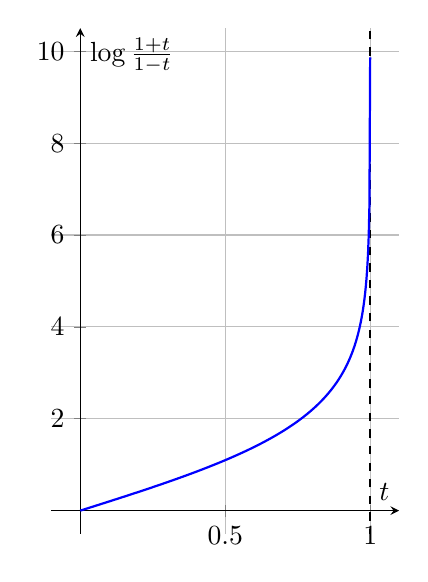
\begin{tikzpicture}
        \begin{axis}[
            domain=0:0.9999, samples=401,
            xlabel={$t$}, ylabel={$\log\frac{1+t}{1-t}$},
            % axis equal,
            axis lines=middle,
            grid=both, 
            width=6cm, height=8cm,
            ymin=-0.5, ymax=10.5, xmin=-0.1, xmax=1.1,
            % restrict y to domain=-50:50, % evita picos numéricos
            % every axis x label/.style={at={(axis description cs:0.95,0.05)},anchor=north east},
            % every axis y label/.style={at={(axis description cs:0.05,0.95)},anchor=south west}
        ]
            % singularidades visuales en t = -1, 1
            % \addplot[dashed, gray] coordinates {(-1,-6) (-1,6)};
            \addplot[thick, dashed] coordinates {(1,-6) (1,12)};
            % función
            \addplot[blue, thick] {ln((1+x)/(1-x))};
            % \addplot[only marks, mark=*, mark options={fill=white}, mark size=0.8pt] coordinates {(0,0)};
        \end{axis}
        \end{tikzpicture}
    \end{figure}
\end{obs}


\begin{ejem}%[de ]
    Consideramos la sucesión $\left(z_n\right)_{n \in \N} \subset \mathbb{D}$ dada por $z_0 = 0$ y de forma recursiva $\forall n \in \N : z_{n} \in [0, 1) : \wp \left(z_n, z_{n-1}\right) = 1$. Entonces, tenemos que
    \[
    \log \frac{1 + \varrho(z_n, z_{n-1})}{1 - \varrho(z_n, z_{n-1})} = 1 \iff \frac{1 + \varrho(z_n, z_{n-1})}{1 - \varrho(z_n, z_{n-1})} = e \iff \varrho(z_n, z_{n-1}) = \frac{e-1}{e+1}.
    \]
    Despejando $z_{n}$, obtenemos que $z_{n} = \tau_{w} (z_{n-1})$ donde $w = \frac{e-1}{e+1}$. Por tanto, $z_n = \tau_w^{n}(0)$.
    
    Por construcción, $\forall n \in \N : \wp(z_n, z_{n-1}) = 1$, luego esta sucesión no es de Cauchy respecto a la métrica de Poincaré. Sin embargo, respecto a la métrica euclídea, tenemos que
    %COMPLETAR
\end{ejem}

% \begin{lem}%REVISAR: muy prescindible porque es obvio
%     Sea $\left(z_n\right)_{n\in\N} \subset \mathbb{D}$ una sucesión, entonces
%     \begin{enumerate}[label=\textnormal{(\arabic*)}]
%         \item $\ds z_n \xrightarrow{n\to\infty} z \in \mathbb{D} \text{ respecto a } \varrho \iff z_n \xrightarrow{n\to\infty} z \text{ respecto a } \wp$.
%         \item $\ds \left(z_n\right)_{n\in\N}$ es de Cauchy respecto a $\varrho \iff \left(z_n\right)_{n\in\N}$ es de Cauchy respecto a $\wp$.
%     \end{enumerate}
% \end{lem}
% \begin{dem}
%     \begin{enumerate}[label=\textnormal{(\arabic*)}]
%         \item Veamos las dos implicaciones:
%         \begin{itemize}
%             \item[$\boxed{\Rightarrow}$] Tenemos que $z_n \xrightarrow{n\to\infty} z$ respecto a $\varrho$, es decir, $\lim_{n\to\infty} \varrho(z_n, z) = 0$. Como $f(t) = \log \frac{1+t}{1-t}$ es continua en $[0,1)$, se tiene que
%             \[
%             \lim_{n\to\infty} \wp(z_n, z) = \lim_{n\to\infty} \log \frac{1 + \varrho(z_n, z)}{1 - \varrho(z_n, z)} = \log \frac{1 + 0}{1 - 0} = \log 1 = 0.
%             \]
%             \item[$\boxed{\Leftarrow}$] Sea $\varepsilon > 0$, entonces $\exists N \in \N : \forall n \geq N : \wp(z_n, z) < \varepsilon$.
%         \end{itemize}
%     \end{enumerate}
% \end{dem}

\begin{teo}%[]\label{teo:}
    $\left(\mathbb{D}, \wp\right)$ es un espacio métrico completo.
\end{teo}
\begin{dem}%REVISAR
    Sea $(z_n)_{n\in\mathbb{N}}\subset\mathbb{D}$ una sucesión de Cauchy para $\wp$.
Definimos $f\colon[0,1)\to[0,\infty)$ por $f(t)=\log\frac{1+t}{1-t}$. Observamos que
$f$ es estrictamente creciente, $f(0)=0$ y satisface $f(t)\to 0 \iff t\to 0$ (en particular tiene inversa creciente
en su imagen).

Para probar completitud tomemos $\varepsilon>0$ arbitrario y pongamos $\eta:=f(\varepsilon)>0$.
Como $(z_n)$ es Cauchy en $\wp$, existe $N$ tal que para todo $m,n\ge N$ se tiene
\[
\wp(z_n,z_m)=f\big(\varrho(z_n,z_m)\big)<\eta.
\]
Dado que $f$ es creciente, de $f(\varrho(z_n,z_m))<f(\varepsilon)$ se sigue
$\varrho(z_n,z_m)<\varepsilon$ para todo $m,n\ge N$. Por tanto $(z_n)$ es una sucesión de Cauchy
en la métrica $\varrho$.

Por hipótesis (ya demostrado en el texto principal) $(\mathbb{D},\varrho)$ es completo, luego
existe $z\in\mathbb{D}$ tal que $\varrho(z_n,z)\to 0$ cuando $n\to\infty$.

Finalmente, usando la propiedad $f(t)\to 0 \iff t\to 0$ y la continuidad de $f$,
se tiene
\[
\wp(z_n,z)=f\big(\varrho(z_n,z)\big)\longrightarrow f(0)=0,
\]
es decir, $z_n\to z$ en la métrica $\wp$. Como toda sucesión de Cauchy en $\wp$ converge en $\mathbb{D}$,
concluimos que $(\mathbb{D},\wp)$ es completo.
\end{dem}

\begin{obs}
    Al igual que ocurría con la métrica pseudohiperbólica, los automorfismos del disco unidad son isometrías para la métrica de Poincaré y podemos reescribir el \hyperref[teo:schwarz-pick]{Teorema de Schwarz-Pick} de la siguiente forma: Sea $f \in \mathcal{S}$, entonces
    \[
    \Big(\forall z, w \in \mathbb{D} : \wp(f(z), f(w)) \leq \wp(z, w)\Big) \we \Big(\wp(f(z), f(w)) = \wp(z, w) \iff f \in \mathrm{Aut} \left(\mathbb{D}\right)\Big). 
    \]
\end{obs}

\begin{defn}[Longitud hiperbólica]\label{defn:longitud-hiperbolica}
    Sea $\gamma \colon [a,b] \to \mathbb{D}$ un camino. La \emph{longitud hiperbólica} de $\gamma$ es
    \[
    \ell(\gamma) = \int_a^b \frac{2\abs{\gamma'(t)}}{1 - \abs{\gamma(t)}^2} \odif{t}.
    \]
\end{defn}
%REVISAR: ¿Por qué esta definición? ¿No tendría más sentido definir la longitud como el supremo de las sumas de distancias respecto a la métrica de Poincaré y luego demostrar que es igual a esta integral?

\begin{lem}%[]\label{lem:}
    Sea $\Gamma \colon [a,b] \to \mathbb{D}$ un camino inyectivo, y $f \in \mathrm{Aut} \left(\mathbb{D}\right)$%REVISAR: ¿Inyectivo por qué?
    \[
    \implies \ell \left(f \circ \Gamma\right) = \ell \left(\Gamma\right). 
    \]
\end{lem}
\begin{dem}
    Como $f \in \mathrm{Aut} \left(\mathbb{D}\right)$ es biyectiva sobre $\mathbb{D}$ y $\Gamma$ es un camino inyectivo en $\mathbb{D}$, entonces $f \circ \Gamma$ también lo es.

    Por el \excref[teo:formula-aut-disco-unidad]{Teo-formula-aut-disco-unidad}, $\exists \gamma \in \mathbb{T}, w \in \mathbb{D} : f = \gamma \, \tau_w$. Por tanto, para el integrando de la longitud hiperbólica de $f \circ \gamma$ se tiene que
    \[
    \frac{\abs{(f \circ \Gamma)'(t)}}{1 - \abs{(f \circ \Gamma)(t)}^2} = \frac{\abs{\gamma} \, \abs{(\tau_w \circ \Gamma)'(t)}}{1 - \abs{\gamma} \, \abs{(\tau_w \circ \Gamma)(t)}^2} = \frac{\abs{(\tau_w \circ \Gamma)'(t)}}{1 - \abs{(\tau_w \circ \Gamma)(t)}^2} = \frac{\abs{\tau_w'(\Gamma(t))} \, \abs{\Gamma'(t)}}{1 - \abs{\tau_w(\Gamma(t))}^2}.
    \]
    Ahora, por el \hyperref[teo:schwarz-pick]{Teorema de Schwarz-Pick}, sabemos que $\tau_w'(z) = \frac{1 - \abs{\tau_w(z)}^2}{1 - \abs{z}^2}$, luego
    \[
    \frac{\abs{(f \circ \Gamma)'(t)}}{1 - \abs{(f \circ \Gamma)(t)}^2} = \frac{\abs{\Gamma'(t)}}{1 - \abs{\Gamma(t)}^2} \implies \ell(f \circ \Gamma) = \ell(\Gamma).
    \]

    \vspace{-\baselineskip}
    \vspace{-\belowdisplayskip}
\end{dem}

\begin{lem}%[]\label{lem:}
    Sea $r \in (0,1)$, entonces $\Gamma_r(t) = t$, $t \in [0, r]$ define el camino más corto respecto a la longitud hiperbólica entre $0$ y $r$. Además, $\ell(\Gamma_r) = \wp(0, r)$.
\end{lem}
\begin{dem}
    Observamos que 
    \[
    \begin{aligned}
        \ell(\Gamma_r) &= \int_0^r \frac{2}{1 - t^2} \odif{t} = \int_{0}^r \left(\frac{1}{1 - t} + \frac{1}{1 + t}\right) \odif{t}\\
        &= -\log(1 - t) + \log(1 + t)\Big|_0^r = \log \frac{1 + r}{1 - r} = \wp(0, r).
    \end{aligned}
    \]

    Sea $\Gamma \colon [0,1] \to \mathbb{D}$ un camino cualquiera entre $0$ y $r$. Podemos integrar en la concatenación de caminos $\Gamma_r^{-1} * \Gamma$ que es un camino cerrado y aplicar el \exhyperref[teo:cauchy-goursat-disco]{Teo-cauchy-goursat-disco}{Teorema de Cauchy-Goursat} a la función $f(z) = \frac{2}{1 - z^2}$, que es holomorfa en $\mathbb{D}$:
    \[
    0 = \int_{\Gamma_r^{-1} * \Gamma} f(z) \odif{z} = \int_{\Gamma} f(z) \odif{z} - \int_{\Gamma_r} f(z) \odif{z} \implies \int_{\Gamma} f(z) \odif{z} = \int_{\Gamma_r} f(z) \odif{z}.
    \]
    Por tanto, se tiene que
    \[
    \ell(\Gamma_r) = \abs{\int_{\Gamma_r} f(z) \odif{z}} = \abs{\int_{\Gamma} f(z) \odif{z}} \leq \int_{\Gamma} \abs{\frac{2}{1 - z^2}} \abs{\odif{z}} 
    \]
    Ahora, por la desigualdad triangular inversa, $\forall z \in \mathbb{D} : \abs{1 - z^2} \geq 1 - \abs{z}^2 > 0$, luego $\frac{1}{\abs{1 - z^2}} \leq \frac{1}{1 - \abs{z}^2}$. Por tanto,
    \[
    \ell(\Gamma_r) \leq \int_{\Gamma} \frac{2}{1 - \abs{z}^2} \abs{\odif{z}} = \ell(\Gamma).
    \]
    Como $\Gamma$ era un camino arbitrario entre $0$ y $r$ y $\Gamma_r$ satisface la igualdad, concluimos que $\Gamma_r$ es el camino más corto entre $0$ y $r$ respecto a la longitud hiperbólica. Falta ver que es único. Si $\Gamma$ satisface la igualdad, entonces todas las desigualdades anteriores se convierten en igualdades, en particular, la desigualdad triangular inversa. Es decir, $\forall z \in \Gamma : \abs{1 - z^2} = 1 - \abs{z}^2$. Esto ocurre si y sólo si $z^2 \in [0,1)$, es decir, si $z \in [0,1)$. Por tanto, el único camino que cumple la igualdad es $\Gamma_r$.
\end{dem}

\begin{obs}
    Por el lema anterior, la longitud hiperbólica entre $0$ y $r \in (0,1)$ viene dada por
    \[
    \wp(0, r) = \ell(\Gamma_r) = \int_0^r \frac{2}{1 - t^2} \odif{t} = \log \frac{1 + r}{1 - r} \xrightarrow[r \to 1^-]{} \infty.
    \]
    Es decir, es como si el borde del disco unidad estuviera a una distancia infinita respecto al origen en la métrica de Poincaré (al menos a lo largo del segmento radial $[0,1)$).
\end{obs}

\begin{teo}%[]\label{teo:}
    Sean $z_1, z_2 \in \mathbb{D}$ distintos, entonces el camino de menor longitud hiperbólica entre $z_1$ y $z_2$ viene dado por $\forall t \in [0,1] : \Gamma(t) =  \tau_{z_1}(\tau_{z_1}(z_2) \, t)$. Además, $\ell(\Gamma) = \wp(z_1, z_2)$.
\end{teo}
\begin{dem}
    Por el ejercicio 8, %ORDENAR referenciar bien
    $f(z) = \bar{\gamma} \, \tau_{z_1}(z)$ con $\gamma = \frac{\tau_{z_1}(z_2)}{\abs{\tau_{z_1}(z_2)}} \in \mathbb{D}$ define un automorfismo del disco unidad que lleva $z_1$ a $0$ y $z_2$ a $\abs{\tau_{z_1}(z_2)}$. Entonces, como los automorfismos del disco unidad son isometrías para la longitud hiperbólica, el camino de menor longitud hiperbólica entre $z_1$ y $z_2$ es $f^{-1} \circ \Gamma_{\abs{\tau_{z_1}(z_2)}}$ donde $\Gamma_{\abs{\tau_{z_1}(z_2)}}$ es el camino más corto entre $0$ y $\abs{\tau_{z_1}(z_2)}$ que viene dado por el lema anterior. %ORDENAR referenciar todo bien
    
    Por tanto, como $f^{-1}(w) = \tau_{z_1}(\gamma \, w)$, se tiene que la parametrización buscada es
     %ORDENAR: referenciar bien (es un ejercicio)
    \[
    \begin{aligned}
        \forall t \in [0, 1] : \Gamma(t) &= f^{-1} \left(\Gamma_{\abs{\tau_{z_1}(z_2)}}(t)\right) = \tau_{z_1} \left(\gamma \, t \abs{\tau_{z_1}(z_2)}\right) = \tau_{z_1} \left(\frac{\tau_{z_1}(z_2)}{\abs{\tau_{z_1}(z_2)}} \, t \abs{\tau_{z_1}(z_2)}\right) \\
        &= \tau_{z_1} \left(\tau_{z_1}(z_2) \, t\right) = \frac{z_1 - \tau_{z_1}(z_2) \, t}{1 - \overline{z_1} \, \tau_{z_1}(z_2) \, t}.
    \end{aligned}
    \] 

    Para calcular su longitud hiperbólica, usamos que los automorfismos del disco unidad son isometrías para la longitud hiperbólica y el lema anterior:
    \[
    \ell(\Gamma) = \ell\left(f \circ \Gamma\right) = \ell\left(\Gamma_{\abs{\tau_{z_1}(z_2)}}\right) = \wp\left(0, \abs{\tau_{z_1}(z_2)}\right) = \wp(z_1, z_2).
    \]

    \vspace{-\baselineskip}
    \vspace{-\belowdisplayskip}
\end{dem}

Este teorema motiva la siguiente definición.

\begin{defn}\label{defn:recta-hiperbolica}
    Sean $z_1, z_2 \in \mathbb{D}$ distintos, $\Gamma$ traza la \textbf{recta hiperbólica} entre $z_1$ y $z_2$
    \[
    \iff \forall t \in \left[0, \abs{\tau_{z_1}(z_2)}\right] : \Gamma(t) = \tau_{z_1} \left(\tau_{z_1}(z_2) \, t\right) \in \mathbb{D}.
    \]
\end{defn}

%COMPLETAR con figura y observación de que las rectas hiperbólicas son arcos de circunferencia ortogonales a la frontera del disco unidad.

\begin{cor}%[]\label{cor:}
    Sean $z_1, z_2, z_3 \in \mathbb{D}$ distintos, entonces están en la misma recta hiperbólica
    \[
    \iff \frac{\tau_{z_1}(z_3)}{\tau_{z_1}(z_2)} \in \R
    \]
\end{cor}
\begin{dem}
    Sabemos que $z_1, z_2, z_3$ están en la misma recta hiperbólica si y sólo si existe $t \in \R$ tal que $z_3 = \tau_{z_1}(\tau_{z_1}(z_2) \, t)$. Aplicando $\tau_{z_1}$ a ambos lados, esto es equivalente a que $\tau_{z_1}(z_3) = \tau_{z_1}(z_2) \, t$. Como $z_2 \neq z_1$ y, por tanto, $\tau_{z_1}(z_2) \neq 0$, esto equivale a que $\frac{\tau_{z_1}(z_3)}{\tau_{z_1}(z_2)} = t \in \R$.
\end{dem}

%COMPLETAR ¿nada de paralelas? REVISAR: mirar ejercicios

\section{Densidad de una métrica}

\begin{defn}[Métrica]\label{defn:metrica}
    Sea $X \neq \varnothing$, $\appl{d}{X \times X}{\R}$ es una métrica $\iff$
    \begin{enumerate}
        \item\label{defn:metrica:positividad} Positividad (no degenerada): $\forall x,y \in X : d(x,y) \geq 0 \we d(x,y) = 0 \iff x = y$.
        \item\label{defn:metrica:simetria} Simetría: $\forall x,y \in X : d(x,y) = d(y,x)$.
        \item\label{defn:metrica:desigualdad-triangular} Desigualdad triangular: $\forall x,y,z \in X : d(x, z) \leq d(x,y) + d(y,z)$.
    \end{enumerate}
    $\forall x, y \in X:$ a la imagen $d(x,y)$ se le llama \textbf{distancia} entre $x$ e $y$.
\end{defn}

% \transclude{desigualdad-triangular-inversa}
\begin{teo}\label{teo:densidad-induce-metrica}
    Sea $\mu \colon \Omega \subset \R^n \to \R$ \exhyperref[defn:continuidad-pnt]{continuidad}{continua} y positiva con $\Omega$ \exhyperref[defn:con-convexo]{con-convexo}{conexo}, definimos
    \[
    \forall \, \Gamma \tex{ \exhyperref[defn:camino]{camino}{camino} inyectivo en } \Omega : \ell_{\mu}(\Gamma) = \int_a^b \mu(\Gamma(t)) \, \exhyperref[defn:norma]{norma}{\norm{\exhyperref[defn:fn-diferenciable-pnt]{fn-diferenciable}{\Gamma'}(t)}} \odif{t}.
    \]
    Entonces, la aplicación $d \colon \Omega \times \Omega \to [0, \infty)$ dada por
    \[
    \forall x, y \in \Omega : d(x, y) = \inf \left\{\ell_{\mu}(\Gamma) : \Gamma \tex{ \exhyperref[defn:camino]{camino}{camino} inyectivo en } \Omega \tex{ entre } x \tex{ e } y\right\},
    \]
    es una \exhyperref[defn:metrica]{metrica}{métrica} en $\Omega$. A la aplicación $\mu$ se le llama la \textbf{densidad métrica} de $d$.
\end{teo} %DEMOSTRACIÓN

\begin{obs}
    El ínfimo en el anterior Teorema se alcanza para cualesquiera dos puntos $x, y \in \Omega$ por alguna curva que los une si y solo si el espacio métrico $(\Omega, d_{\mu})$ es \exhyperref[defn:espacio-metrico-completo]{Completo}{completo}. 
\end{obs}

% También podemos permitir que $\mu$ tenga singularidades aisladas en puntos de $\Omega$, es decir, que $\mu$ tome el valor infinito en dichos puntos, siempre que exista un camino entre dos puntos cualesquiera de $\Omega$ que evite esas singularidades y tenga longitud finita.

\subsection{Densidad métrica inducida por una aplicación holomorfa}

\begin{defn}[Densidad métrica inducida]\label{defn:densidad-metrica-inducida}
    Sea $\mu \colon \Omega \subset \C \to (0, \infty)$ una \exhyperref[teo:densidad-induce-metrica]{teo-densidad-induce-metrica}{densidad métrica} en un dominio $\Omega$ y sea $f \colon \Omega_1 \subset \C \to \Omega$ una \exhyperref[defn:fn-holomorfa]{fn-holomorfa}{función holomorfa}, $f^*\mu \colon \Omega_1 \to \R$ es la densidad métrica inducida por $f$ y $\mu$ en $\Omega_1$
    \[
    \iff \forall z \in \Omega_1 : (f^* \mu)(z) = \mu(f(z)) \, \abs{f'(z)}.
    \]
\end{defn}

\begin{obs}\label{obs:longitud-camino-densidad-metrica-inducida}
    Entonces, para $\Gamma$ un camino inyectivo en $\Omega_1$, se tiene que
    \[
    \ell_{f^* \mu} (\Gamma) = \int_a^b (f^* \mu)(\Gamma(t)) \, \abs{\Gamma'(t)} \odif{t} = \int_a^b \underbrace{\mu(f(\Gamma(t)))}_{\mu \left(\left(f \circ \Gamma\right)(t)\right)} \, \underbrace{\abs{f'(\Gamma(t))} \, \abs{\Gamma'(t)}}_{\abs{(f \circ \Gamma)'(t)}} \odif{t} = \ell_{\mu} (f \circ \Gamma).
    \]
\end{obs}

\begin{obs}
    En el \textbf{caso particular} en el que $\Omega_1 = \Omega_2 = \Omega$, podemos comparar $(f^*\mu)$ y $\mu$ en cualquier punto de $\Omega$. Por ejemplo, si $\forall z \in \Omega : (f^* \mu)(z) \leq \mu(z)$, entonces $\forall \Gamma$ camino en $\Omega : \ell_{f^* \mu}(\Gamma) \leq \ell_{\mu}(\Gamma)$ y, por tanto, $\forall x, y \in \Omega : d_{f^* \mu}(x, y) \leq d_{\mu}(x, y)$.
    
    Ahora bien, como $\forall \Gamma$ camino en $\Omega$ entre $z$ y $w : f \circ \Gamma$ es un camino en $\Omega$ entre $f(z)$ y $f(w)$, se tiene que
    \[
    \begin{aligned}
        d_{\mu}(f(z), f(w)) &= \inf \left\{\ell_{\mu}(\Gamma') : \Gamma' \tex{ camino en } \Omega \tex{ entre } f(z) \tex{ y } f(w)\right\} \\
        &\leq \inf \left\{\ell_{\mu}(f \circ \Gamma) : \Gamma \tex{ camino en } \Omega \tex{ entre } z \tex{ y } w\right\} = d_{f^* \mu}(z, w).
    \end{aligned}
    \]
    Por tanto, $\forall z, w \in \Omega : d_{\mu}(f(z), f(w)) \leq d_{\mu}(z, w)$ y $f$ es una contracción respecto a $d_{\mu}$.
    
    Concretamente, para la métrica de Poincaré en el disco unidad, la densidad métrica es $\mu(z) = \frac{2}{1 - \abs{z}^2}$. Entonces, si $f \in \mathcal{S}$, por el \hyperref[teo:schwarz-pick]{Teorema de Schwarz-Pick}, se tiene que
    \[
    \forall z \in \mathbb{D} : (f^* \mu)(z) = \frac{2}{1 - \abs{f(z)}^2} \, \abs{f'(z)} \leq \frac{2}{1 - \abs{z}^2} = \mu(z).
    \]
    En consecuencia, $f$ es una contracción respecto a la métrica de Poincaré:%ORDENAR: referenciar observación donde se ve esto
    \[
    \forall z, w \in \mathbb{D} : \wp(f(z), f(w)) \leq \wp(z, w).
    \]
\end{obs}

\subsection{Curvatura de una densidad métrica}

La curvatura gaussiana $\kappa_\mu \colon \Omega \to \R$ asociada a una densidad métrica $\mu \colon \Omega \to (0, \infty)$ viene dada por la fórmula
\[
\forall z \in \Omega : \kappa_\mu(z) = -\frac{B_{\varrho} (\log \mu)(z)}{\mu(z)^2}.
\]
Para una explicación más detallada del origen de esta fórmula, véase \cite{krantzComplexAnalysisGeometric2004}, Anexo.

Para la métrica de Poincaré en el disco unidad, tenemos que
\[
\begin{aligned}
    B_{\varrho} \log \mu (z) &= B_{\varrho} \log \left(\frac{2}{1 - \abs{z}^2}\right) = 4 \,\pdv{}{z} \pdv{}{\bar{z}} \left(\log 2 - \log(1 - z \bar{z})\right) \\
    &= -4 \,\pdv{}{z} \left(\frac{-z}{1 - z \bar{z}}\right) = 4 \, \frac{1 - z \bar{z} - z \left(- \bar{z}\right)}{(1 - z \bar{z})^2} = \frac{4}{{\left(1 - \abs{z}^2\right)}^2}.
\end{aligned}
\]
Observamos que $(\mu(z))^2 = \left(\frac{2}{1 - \abs{z}^2}\right)^2 = \frac{4}{{\left(1 - \abs{z}^2\right)}^2}$, luego
\[
B_{\varrho} \log \mu (z) = (\mu(z))^2 \implies \kappa_\mu(z) = - \frac{B_{\varrho} \log \mu (z)}{(\mu(z))^2} = -1.
\] 

Una de las propiedades más importantes de la curvatura es que es conformalmente invariante, es decir, se conserva al considerar la densidad métrica inducida por una aplicación conforme (holomorfa con derivada no nula). Más concretamente, tenemos el siguiente resultado.

\begin{lem}[Curvatura de la métrica inducida]\label{lem:curvatura-pullback}
    Sea $f\colon \Omega_1\to\Omega_2$ holomorfa y sea $\sigma$ una densidad métrica $\mathcal{C}^2$
    \[
        \implies \forall z \in \Omega_1 : f'(z) \neq 0 : \kappa_{f^*\sigma}(z)=\kappa_{\sigma}\big(f(z)\big).
    \]
\end{lem}   
\begin{dem}
    Por definición de $f^*\sigma$, tenemos que $\log(f^*\sigma) = \log(\sigma\circ f) + \log \abs{f'}$.
    Como $f'$ es holomorfa, en cualquier punto donde $f'\neq0$ la función $f'$ no se anula localmente y $\log\abs{f'}$ es armónica, por tanto $B_{\varrho}\log\abs{f'} = 0$. %REVISAR no entiendo bien esto
    Además, por el \excref[lem:laplaciano-cambio-variable]{Lem-laplaciano-cambio-variable}, tenemos que
    \[
        B_{\varrho}\log(f^*\sigma)(z) = B_{\varrho} \log(\sigma\circ f)(z) + \cancelto{0}{B_{\varrho}\log\abs{f'}(z)} = \abs{f'(z)}^2 \big(B_{\varrho}\log\sigma\big)(f(z)).
    \]
    Usando la definición de curvatura y que $(f^*\sigma)(z)^2 = \sigma(f(z))^2\,\abs{f'(z)}^2$ se obtiene
    \[
        \kappa_{f^*\sigma}(z) = - \frac{B_{\varrho}\log(f^*\sigma)(z)}{(f^*\sigma)(z)^2} = - \frac{\abs{f'(z)}^2 \, (B_{\varrho}\log\sigma )(f(z))}{\sigma(f(z))^2 \, \abs{f'(z)}^2} = \kappa_{\sigma}(f(z)).
    \]

    \vspace{-\baselineskip}
    \vspace{-\belowdisplayskip}
\end{dem}

Ahlfors enunció el Lema de Schwarz como un resultado acerca de la curvatura.

\begin{lem}%[]\label{lem:}
    Sea $\Omega \subset \C$ un dominio dotado de una densidad métrica $\sigma$ tal que $\kappa_{\sigma}(z) \leq -1$ para todo $z \in \Omega$. Sea $f \colon \mathbb{D} \to \Omega$ una aplicación holomorfa, entonces
    \[
    \forall z \in \mathbb{D} : \left(f^* \sigma\right) (z) \leq \mu(z)
    \]
    donde $\mu$ es la densidad métrica de la métrica de Poincaré en $\mathbb{D}$.
\end{lem}
\begin{dem}
    Sea $r \in (0,1)$. En el disco $D_r(0)$, la función dada por $\mu_r(z) = \frac{2}{r^2 - \abs{z}^2}$ está bien definida. Además, es una densidad métrica en $D_r(0)$ cuya curvatura es $\kappa_{\mu_r}(z) = -1$ para todo $z \in D_r(0)$ (el cálculo es análogo al realizado para $\mu$).

    Definimos la función $\phi \colon D_r(0) \to \R$ mediante $\forall z \in D_r(0) : \phi(z) = \frac{(f^* \sigma)(z)}{\mu_r(z)}$. Entonces, $\phi \geq 0$ y como $\mu_r$ no se anula y $f^* \sigma$ es continua, $\phi$ es continua en $D_r(0)$. Además, tenemos que
    \[
    \lim_{\abs{z} \to r^-} \phi(z) = \lim_{\abs{z} \to r^-} \frac{(f^* \sigma)(z)}{\mu_r(z)} = \lim_{\abs{z} \to r^-} (f^* \sigma)(z) \cdot \frac{r^2 - \abs{z}^2}{2} = 0.
    \]
    Por tanto, $\phi$ alcanza su máximo $M$ en un punto $z_0 \in \bar{D_r(0)}$ y, para probar el teorema, basta ver que $M \leq 1$.
    
    Si el máximo se alcanza en la frontera, entonces $M = \phi(z_0) = 0 \leq 1$ y el resultado se cumple. Suponemos que el máximo se alcanza en el interior, es decir, $z_0 \in D_r(0)$, podemos suponer además que $\phi(z_0) > 0$, es decir, $f^* \sigma (z_0) > 0$. Como $\phi$ es $\mathcal{C}^2$ en un entorno de $z_0$ (pues $f^* \sigma$ y $\mu_r$ lo son), podemos aplicar el operador laplaciano en $z_0$ y obtener que $B_{\varrho} \log \phi(z_0) \leq 0$ (pues $z_0$ es un máximo local y $\log$ es creciente). %REVISAR esta última afirmación esto es porque la parte real/imaginaria de una función holomorfa es armónica %ORDENAR: escribir en lema y demostrarlo y citarlo
    Por tanto, tenemos que
    \[
    \begin{aligned}
        B_{\varrho} \log \phi (z_0) &= B_{\varrho} \log (f^* \sigma)(z_0) - B_{\varrho} \log \mu_r (z_0) \\
        &= - \kappa_{f^* \sigma}(z_0) \, (f^* \sigma(z_0))^2 + \kappa_{\mu_r}(z_0) \, (\mu_r(z_0))^2 \leq 0.
    \end{aligned}
    \]
    Ahora bien, por el lema anterior, %ORDENAR referenciar
    $\kappa_{f^* \sigma}(z) = \kappa_{\sigma}(f(z)) \leq -1$ para todo $z \in \mathbb{D}$ y $\kappa_{\mu_r}(z) = -1$ para todo $z \in D_r(0)$. Por tanto, como $\kappa_{\mu_r} (z_0) (\mu_r(z_0))^2 \leq \kappa_{f^* \sigma}(z_0) (f^* \sigma(z_0))^2$,
    \[
    - (\mu_r(z_0))^2 \leq \kappa_{\sigma} (f(z_0)) (f^* \sigma(z_0))^2 \leq - (f^* \sigma(z_0))^2 \implies \frac{(f^* \sigma)(z_0)}{\mu_r(z_0)} \leq 1.
    \]
    Haciendo ahora tender $r$ a $1$ se tiene que $\forall z \in \mathbb{D} : (f^* \sigma)(z) \leq \mu(z)$.
     %COMPLETAR
\end{dem}

\begin{obs}
    Este resultado generaliza el \hyperref[teo:schwarz-pick]{Teorema de Schwarz-Pick}, ya que si tomamos $\Omega = \mathbb{D}$ con la métrica de Poincaré ($\sigma = \mu$), entonces $\kappa_{\sigma}(z) = -1 \leq -1$ para todo $z \in \mathbb{D}$ y recuperamos la segunda desigualdad:
    \[
    \forall z \in \mathbb{D} : (f^* \mu)(z) = \mu(f(z)) \, \abs{f'(z)} = \frac{2}{1 - \abs{f(z)}^2} \, \abs{f'(z)} \leq \frac{2}{1 - \abs{z}^2} = \mu(z).
    \]
    Y esta desigualdad, a su vez, implica la primera por la discusión previa sobre densidades métricas inducidas.
\end{obs}

%REVISAR COMPLETAR: mirarse \cite{krantzComplexAnalysisGeometric2004} capítulo 2 y \cite{pressleyElementaryDifferentialGeometry2012}

\section{Métrica hiperbólica en el semiplano superior}

Recordemos que el semiplano superior es el conjunto $\mathbb{H} = \{z \in \C : \Im(z) > 0\}$. En lugar de empezar de nuevo desde cero, vamos a usar el hecho de que el semiplano superior es conformemente equivalente al disco unidad mediante la transformación de Möbius $\varphi \colon \mathbb{H} \to \mathbb{D}$ dada por 
\[
\forall z \in \mathbb{H} : \varphi(z) = \frac{z - i}{z + i}.
\]
Entonces, esta transformación es una biyección holomorfa de $\mathbb{H}$ sobre $\mathbb{D}$ con inversa también holomorfa dada por
\[
\forall w \in \mathbb{D} : \varphi^{-1}(w) = i \, \frac{1 + w}{1 - w}.
\]

Usando la \hyperref[defn:densidad-metrica-inducida]{definición de densidad métrica inducida}, podemos definir la densidad métrica en $\mathbb{H}$ inducida por la métrica de Poincaré en $\mathbb{D}$ mediante la transformación $\varphi$:
\[
\mu_{\mathbb{H}}(z) = \left(\varphi^* \mu\right)(z) = \mu(\varphi(z)) \, \abs{\varphi'(z)}.
\]
Calculamos primero la derivada de $\varphi$:
\[
\forall z \in \mathbb{H} : \varphi'(z) = \frac{(z + i) - (z - i)}{(z + i)^2} = \frac{2i}{(z + i)^2} \implies \abs{\varphi'(z)} = \frac{2}{\abs{z + i}^2}.
\]
% Por otro lado, tenemos que
% \[
% \abs{\varphi(z)}^2 = \frac{\abs{z - i}^2}{\abs{z + i}^2} = \frac{(z -i) (\bar{z} + i)}{(z + i)(\bar{z} - i)} = \frac{\abs{z}^2 + 1 - 2 \Im(z)}{\abs{z}^2 + 1 + 2 \Im(z)}.
% \]

Por tanto, nos queda que
\[
\begin{aligned}
    \forall z \in \mathbb{H} : \mu_{\mathbb{H}}(z) &= \frac{2}{1 - \abs{\varphi(z)}^2} \cdot \frac{2}{\abs{z + i}^2} = \frac{4}{\abs{z + i}^2 - \abs{z - i}^2} \\
    &= \frac{4}{(z + i)(\overline{z} - i) - (z - i)(\overline{z} + i)} = \frac{4}{2i(z - \overline{z})} = \frac{2}{\Im(z)}.
\end{aligned}
\]

Por el ejercicio 2, %ORDENAR: referenciar bien
tenemos que los espacios métricos $(\mathbb{D}, \wp)$ y $(\mathbb{H}, d_{\mu_{\mathbb{H}}})$ son isométricos mediante la transformación $\varphi$. Por tanto, podemos definir la métrica hiperbólica en el semiplano superior como la métrica $d_{\mu_{\mathbb{H}}}$ inducida por la densidad métrica $\mu_{\mathbb{H}}(z) = \frac{2}{\Im(z)}$ que es el pullback de la métrica de Poincaré en el disco unidad mediante la transformación $\varphi$.

\begin{obs}
    Dado que las rectas hiperbólicas en el disco unidad son arcos de circunferencia ortogonales a $\mathbb{T}$ y $\varphi$ es una transformación de Möbius (manda circunferencias generalizadas en circunferencias generalizadas y preserva ángulos), las rectas hiperbólicas en el semiplano superior son imágenes mediante $\varphi^{-1}$ de dichos arcos, es decir, son semicircunferencias ortogonales a la recta real y rectas perpendiculares a la recta real puesto que $\varphi(\mathbb{T}) = \R \cup \{\infty\}$.
\end{obs}

\section{Métrica esférica en el plano complejo extendido}

La métrica esférica en el plano complejo extendido $\widehat{\C} = \C \cup \{\infty\}$ se define mediante la densidad métrica $\mu_{\mathrm{esf}} \colon \widehat{\C} \to (0, \infty)$ dada por
\[
\forall z \in \C : \mu_{\mathrm{esf}}(z) = \frac{2}{1 + \abs{z}^2} \quad\we \quad \mu_{\mathrm{esf}}(\infty) = 0.
\]
Esta densidad métrica es la pullback de la métrica estándar en la esfera unidad mediante la proyección estereográfica $\pi \colon \widehat{\C} \to S^2$ dada por
\[
\forall z \in \C : \pi(z) = \left(\frac{2 \Re(z)}{1 + \abs{z}^2}, \frac{2 \Im(z)}{1 + \abs{z}^2}, \frac{\abs{z}^2 - 1}{1 + \abs{z}^2}\right) \quad\we\quad \pi(\infty) = (0, 0, 1).
\]

\section{Ejercicios}

\begin{ejer}
    Demuestra que la métrica de Poincaré $\wp$ satisface que
    \[
    \forall z, w \in \mathbb{D} : \wp(z, w) = 2 \tanh^{-1} \abs{\frac{z - w}{1 - \overline{w}z}}.
    \]
\end{ejer}
\begin{sol}
    Recordemos la definición de la tangente hiperbólica:
    \[
    \tanh(z) = \frac{\sinh(x)}{\cosh(x)} = \frac{e^x - e^{-x}}{e^x + e^{-x}} = \frac{e^{2x} - 1}{e^{2x} + 1}.
    \]
    Entonces, despejando, tenemos que $e^{2x} \left(1 - \tanh(x)\right) = 1 + \tanh(x)$, luego
    \[
    e^{2x} = \frac{1 + \tanh(x)}{1 - \tanh(x)} \implies \tanh^{-1}(y) = \frac{1}{2} \, \log \frac{1 + y}{1 - y}.
    \]
    En particular, para $y = \varrho (z, w)$ con $z, w \in \mathbb{D}$, tenemos que
    \[
    \tanh^{-1} \left(\varrho(z, w)\right) = \frac{1}{2} \, \log \frac{1 + \varrho(z, w)}{1 - \varrho(z, w)} = \frac{1}{2} \, \wp(z, w)
    \]
    por definición de la métrica de Poincaré. Por tanto, como $\varrho(z, w) = \abs{\frac{z - w}{1 - \overline{w} z}}$, se tiene que
    \[
    \implies \wp(z, w) = 2 \, \tanh^{-1} \left(\varrho(z, w)\right) = 2 \, \tanh^{-1} \abs{\frac{z - w}{1 - \overline{w} z}}.
    \]

    \vspace{-\baselineskip}
    \vspace{-\belowdisplayskip}
    \hfill\qedsymbol
\end{sol}

\begin{ejer}
    Sea $f \colon \Omega_1 \to \Omega_2$ una aplicación holomorfa entre dos dominios $\Omega_1, \Omega_2 \subset \C$ dotados de densidades métricas $\mu_1, \mu_2$ respectivamente. Demuestra que
    \[
    f \tex{ es una isometría entre } (\Omega_1, d_{\mu_1}) \tex{ y } (\Omega_2, d_{\mu_2}) \iff \forall z \in \Omega_1 : (f^* \mu_2)(z) = \mu_1(z).
    \]
\end{ejer}
\begin{sol}
    Veamos ambas implicaciones por separado:
    \begin{itemize}
        \item[$\boxed{\Rightarrow}$]
        \item[$\boxed{\Leftarrow}$] 
    \end{itemize}
\end{sol}
%DEMOSTRACIÓN

\begin{ejer}%EJERCICIO 
    Demuestra que la curvatura de la métrica esférica es constante e igual a $+1$.
\end{ejer}
\begin{sol}

\end{sol}

%COMPLETAR mirar Geometry: Euclid and Beyond.

% 3.1 y 3.2 para el jueves 20 de noviembre


    %%%% Final del cuerpo %%%%%%%%%%
    % Apéndices (Opcionales)
    \appendix 
    \chapter{Resultados auxiliares}
    En este apéndice recopilamos algunas definiciones y lemas auxiliares que se utilizan a lo largo del texto. Aunque la mayoría de estos resultados son bien conocidos, los incluimos aquí para mayor claridad y comodidad del lector. Comenzamos con una desigualdad elemental que será empleada repetidamente en las demostraciones de los teoremas principales.

    \begin{lem}[Desigualdad básica]
    Sean $a,b \in \mathbb{R}$ con $b \neq 0$. Entonces
    \[
    \left| \frac{a}{b} \right| \leq \frac{|a|}{|b|}.
    \]
    Además, la igualdad se cumple si y solo si $ab \geq 0$.
    \end{lem}

    \begin{proof}
    La prueba se deduce directamente de la propiedad multiplicativa del valor absoluto, es decir, $|ab| = |a||b|$ para todo $a,b \in \mathbb{R}$. Dividiendo ambos lados por $|b|^2$ obtenemos la desigualdad. La caracterización de la igualdad es inmediata.
    \end{proof}


    \chapter{Otro apéndice}


    %%%La bibliografía
    \begin{thebibliography}{10}
        \addcontentsline{toc}{chapter}{\bibname}

        \bibitem{Abel} 
            \textsc{N.\,H. Abel},
            Beweis eines Ausdrucks, von welchem die Binomial-Formel ein einzelner Fall ist. 
            \textit{J. Reine angew. Math.} {\bf1} (1826), 159--160.

        \bibitem{S-W}
            \textsc{E.\,M. Stein y G. Weiss},
            \textit{Introduction to  Fourier analysis on Euclidean spaces.}
            Princeton Mathematical Series~32, Princeton University Press, Princeton, NJ, 1971.
        
    \end{thebibliography}
    \cleardoublepage
\end{document}
